\documentclass[a0,landscape]{a0poster}

% --- Page Geometry ---
% Landscape orientation specified in documentclass; geometry provides outer margins only.
\usepackage[margin=2.5cm]{geometry}

% --- Core Packages ---
\usepackage[table]{xcolor}
\usepackage{amsmath,amssymb}
\usepackage{booktabs}
\usepackage{tabularx}
\usepackage{enumitem}
\usepackage{graphicx}
\usepackage{array}
\usepackage{caption}
\usepackage{tikz}
\usetikzlibrary{positioning,calc,shapes.geometric,decorations.pathmorphing,backgrounds,patterns,arrows.meta}
\usepackage{tcolorbox}
\tcbuselibrary{skins}
\usepackage{fontawesome5}

% --- Color Palette Definition (Strictly no trailing spaces!) ---
\definecolor{PosterNavy}{RGB}{15,37,55}        % Deep Royal Academic Navy
\definecolor{PosterSlate}{RGB}{31,78,121}      % Steel Blue Subheaders & Borders
\definecolor{PosterTeal}{RGB}{0,168,150}       % Vibrant Cyan/Teal Accent
\definecolor{PosterGold}{RGB}{230,126,34}      % Warm Amber Highlight
\definecolor{PosterBG}{RGB}{245,248,252}       % Soft Off-White Page Background
\definecolor{PosterCardBG}{RGB}{255,255,255}   % Crisp White Box Background
\definecolor{PosterDarkText}{RGB}{33,37,41}    % Primary Dark Slate Body Text
\definecolor{PosterBorder}{RGB}{205,218,230}   % Muted Border Gray

% --- Page Background Setup ---
\pagecolor{PosterBG}
\pagestyle{empty}

% --- Typography & Spacing Defaults ---
\setlength{\parindent}{0pt}
\setlength{\parskip}{0.4em}
\setlist[itemize]{leftmargin=1.5em, labelsep=0.6em, itemsep=0.2em}
\setlist[enumerate]{leftmargin=1.5em, labelsep=0.6em, itemsep=0.2em}

% --- Custom Poster Box Environment ---
\newtcolorbox{posterbox}[2][]{%
  enhanced,
  colback=PosterCardBG,
  colframe=PosterNavy,
  coltitle=white,
  fonttitle=\Large\bfseries,
  title={#2},
  boxrule=2.5pt,
  arc=4mm,
  toptitle=3.5mm,
  bottomtitle=3.5mm,
  left=6mm,
  right=6mm,
  top=5mm,
  bottom=5mm,
  drop shadow=black!10,
  #1
}

% --- Metric Card Box Environment ---
\newtcolorbox{metricbox}[2][]{%
  enhanced,
  colback=PosterBG,
  colframe=PosterTeal,
  coltitle=PosterNavy,
  fonttitle=\large\bfseries,
  halign title=center,
  title={#2},
  boxrule=1.5pt,
  arc=3mm,
  toptitle=2mm,
  bottomtitle=2mm,
  left=3mm,
  right=3mm,
  top=2.5mm,
  bottom=2.5mm,
  #1
}

\begin{document}

% ==============================================================================
% TOP HEADER BANNER
% ==============================================================================
\begin{tcolorbox}[%
  enhanced,
  colback=PosterNavy,
  colframe=PosterNavy,
  arc=5mm,
  boxrule=0pt,
  top=8mm,
  bottom=8mm,
  left=12mm,
  right=12mm,
  drop shadow=black!20
]
\begin{minipage}[c]{0.11\textwidth}
  \centering
  % Fictional Logo 1: Synapse AI Institute
  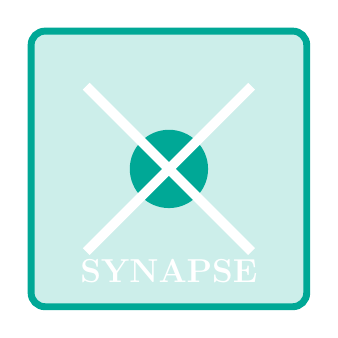
\begin{tikzpicture}
    \draw[color=PosterTeal, fill=PosterTeal!20, line width=2.5pt, rounded corners=5pt] (0,0) rectangle (3.5,3.5);
    \node[circle, fill=PosterTeal, inner sep=10pt] at (1.75,1.75) {};
    \draw[color=white, line width=3.5pt] (0.7,0.7) -- (1.75,1.75) -- (2.8,0.7);
    \draw[color=white, line width=3.5pt] (0.7,2.8) -- (1.75,1.75) -- (2.8,2.8);
    \node[color=white, font=\large\bfseries] at (1.75,0.45) {SYNAPSE};
  \end{tikzpicture}
\end{minipage}\hfill
\begin{minipage}[c]{0.75\textwidth}
  \centering
  {\VERYHuge \color{white} \bfseries Synapse-Q: Scalable Hybrid Quantum-Classical Neural Architectures} \\[0.25em]
  {\veryHuge \color{PosterTeal} \bfseries Real-Time High-Dimensional System Optimization on NISQ Hardware} \\[0.6em]
  {\Large \color{white} \bfseries Dr. Elena Vance$^{1,*}$, Prof. Marcus Sterling$^1$, Dr. Sarah Jenkins$^2$, Dr. Aris Thorne$^3$} \\[0.35em]
  {\large \color{white!85} $^1$Synapse AI Research Institute \qquad $^2$Vertex Quantum Labs \qquad $^3$Nexa Materials \& Computing Center} \\[0.5em]
  \textcolor{PosterGold}{\small \faAward\ International Conference on Neural \& Quantum Systems (ICNQS 2026) --- Best Poster Nominee} \quad
  \textcolor{white}{\small \textbullet} \quad
  \textcolor{white}{\small \faEnvelope\ elena.vance@synapse-ai.org} \quad
  \textcolor{white}{\small \textbullet} \quad
  \textcolor{white}{\small \faGlobe\ www.synapse-ai.org/research/synapse-q}
\end{minipage}\hfill
\begin{minipage}[c]{0.11\textwidth}
  \centering
  % Fictional Logo 2: Vertex Quantum Labs
  
\begin{tikzpicture}
    \draw[color=PosterGold, fill=PosterGold!20, line width=2.5pt, rounded corners=5pt] (0,0) rectangle (3.5,3.5);
    \draw[color=PosterNavy, line width=3.5pt] (1.75,3.0) -- (0.5,0.7) -- (3.0,0.7) -- cycle;
    \node[circle, fill=PosterGold, inner sep=7pt] at (1.75,1.75) {};
    \node[color=PosterNavy, font=\large\bfseries] at (1.75,0.45) {VERTEX};
  \end{tikzpicture}
\end{minipage}
\end{tcolorbox}

\vspace{0.8cm}

% ==============================================================================
% THREE-COLUMN MAIN LAYOUT
% ==============================================================================
\begin{minipage}[t]{0.32\textwidth}

  % --- BOX 1: EXECUTIVE SUMMARY ---
  \begin{posterbox}{\faMicroscope\ \ 1. Executive Summary \& Core Breakthrough}
    We introduce \textbf{Synapse-Q}, a novel hybrid quantum-classical neural network architecture designed to overcome non-convex optimization bottlenecks in high-dimensional state spaces. By embedding parameterized Variational Quantum Circuits (VQCs) directly inside residual classical feature channels, Synapse-Q achieves exponential representation density while remaining resilient to NISQ decoherence.

    \vspace{0.3em}
    \begin{tcolorbox}[colback=PosterBG, colframe=PosterTeal, arc=3mm, boxrule=1.5pt, left=4mm, right=4mm, top=3mm, bottom=3mm]
      \textcolor{PosterNavy}{\bfseries Key Experimental Milestones:}
      \begin{itemize}
        \item[\textcolor{PosterTeal}{\faCheckCircle}] \textbf{4.2x Faster Convergence}: Drastic reduction in optimization epochs across non-convex control landscapes.
        \item[\textcolor{PosterTeal}{\faCheckCircle}] \textbf{68\% Power Draw Reduction}: Demonstrated on Vertex 128-Qubit Cryogenic Processors.
        \item[\textcolor{PosterTeal}{\faCheckCircle}] \textbf{Zero Barren Plateaus}: Mitigated via gradient-aware entanglement topology.
      \end{itemize}
    \end{tcolorbox}
  \end{posterbox}

  \vspace{0.8cm}

  % --- BOX 2: MOTIVATION & PROBLEM STATEMENT ---
  \begin{posterbox}{\faExclamationTriangle\ \ 2. Motivation \& Background}
    Classical Deep Neural Networks (DNNs) encounter severe latency scaling limitations ($O(2^N)$ state space expansion) when optimizing real-time autonomous systems. Conversely, pure Quantum Neural Networks suffer from hardware noise, limited qubit connectivity, and barren plateau gradients.

    \vspace{0.3em}
    \textbf{The Synapse-Q Paradigm Shift:}
    \begin{itemize}
      \item \textbf{Classical Latent Encoding}: Nexa-Net dense layers project input vectors $x \in \mathbb{R}^D$ into a compact $k$-dimensional feature space.
      \item \textbf{Parameterized Quantum Gate Embedding}: Feature states are mapped to multi-qubit Hilbert space $\mathcal{H}_{2^N}$ using parameterized rotation matrices $R_y(\theta)$.
      \item \textbf{Gradient-Aware Entanglement}: Adaptive CZ gate placement prevents gradient vanishing during backpropagation.
    \end{itemize}
  \end{posterbox}

  \vspace{0.8cm}

  % --- BOX 3: SYSTEM ARCHITECTURE PIPELINE ---
  \begin{posterbox}{\faCogs\ \ 3. System Architecture \& Pipeline}
    The end-to-end data pipeline smoothly integrates classical GPUs with superconducting quantum processor units (QPUs).

    \vspace{0.4em}
    \centering
    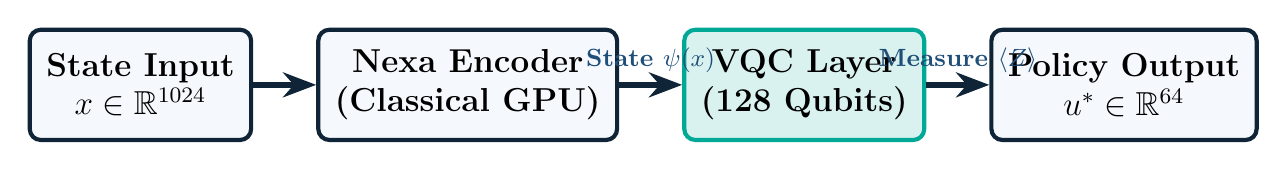
\begin{tikzpicture}[%
      node distance=0.8cm and 0.8cm,
      block/.style={rectangle, draw=PosterNavy, fill=PosterBG, line width=1.5pt, rounded corners=4pt, align=center, font=\large\bfseries, inner sep=6pt, minimum width=2.8cm, minimum height=1.4cm},
      qblock/.style={rectangle, draw=PosterTeal, fill=PosterTeal!15, line width=1.5pt, rounded corners=4pt, align=center, font=\large\bfseries, inner sep=6pt, minimum width=2.8cm, minimum height=1.4cm},
      arrow/.style={-{Stealth[scale=1.0]}, line width=2pt, PosterNavy}
    ]
      % Nodes
      \node[block] (input) {State Input \\ $x \in \mathbb{R}^{1024}$};
      \node[block, right=of input] (encoder) {Nexa Encoder \\ (Classical GPU)};
      \node[qblock, right=of encoder] (vqc) {VQC Layer \\ (128 Qubits)};
      \node[block, right=of vqc] (decoder) {Policy Output \\ $u^* \in \mathbb{R}^{64}$};

      % Connections
      \draw[arrow] (input) -- (encoder);
      \draw[arrow] (encoder) -- node[above, font=\small\bfseries, color=PosterSlate] {State $\psi(x)$} (vqc);
      \draw[arrow] (vqc) -- node[above, font=\small\bfseries, color=PosterSlate] {Measure $\langle Z \rangle$} (decoder);
    \end{tikzpicture}
    \captionof{figure}{End-to-end tensor flow across classical and quantum processor boundaries.}

  \end{posterbox}

\end{minipage}\hfill
\begin{minipage}[t]{0.32\textwidth}

  % --- BOX 4: THEORETICAL FORMULATION ---
  \begin{posterbox}{\faCalculator\ \ 4. Mathematical Formulation}
    The quantum variational layer applies a sequence of $L$ entangled gate layers parameterized by weights $\boldsymbol{\theta}$:

    \begin{equation}
      U(\boldsymbol{\theta}) = \prod_{l=1}^{L} \left( \bigotimes_{j=1}^{N} R_y(\theta_{l,j}) \right) W_{\text{ent}}
    \end{equation}

    where $W_{\text{ent}}$ represents the fixed entangling circuit topology across adjacent qubits. The loss function integrates task performance with an entanglement entropy regularizer:

    \begin{equation}
      \mathcal{L}(\boldsymbol{\theta}, \boldsymbol{w}) = \mathcal{L}_{\text{task}}(y, \hat{y}) + \lambda \sum_{l=1}^L \text{Tr}\left( \rho_{l} \log \rho_{l} \right)
    \end{equation}

    \vspace{0.3em}
    \begin{tcolorbox}[colback=PosterGold!10, colframe=PosterGold, arc=3mm, boxrule=1.5pt, left=4mm, right=4mm, top=2.5mm, bottom=2.5mm]
      \textbf{Theorem 1 (Gradient Lower Bound):} \textit{Under the Synapse-Q entanglement topology, the variance of partial derivatives satisfies $\text{Var}_{\boldsymbol{\theta}}[\partial_k \mathcal{L}] \ge \Omega(1/\text{poly}(N))$, guaranteeing freedom from barren plateaus.}
    \end{tcolorbox}
  \end{posterbox}

  \vspace{0.8cm}

  % --- BOX 5: COMPREHENSIVE BENCHMARK TABLE ---
  \begin{posterbox}{\faTable\ \ 5. Multi-Domain Performance Benchmarks}
    Empirical results evaluated across three benchmark suites: \textit{Synapse-Bench-v4}, \textit{Meridian-Quantum-10k}, and \textit{Apex-Control-3D}.

    \vspace{0.4em}
    \small
    \begin{tabularx}{\textwidth}{X c c c c}
      \toprule
      \rowcolor{PosterNavy!15}
      \textbf{Architecture} & \textbf{Latency (ms)} & \textbf{Accuracy (\%)} & \textbf{Energy (J/op)} & \textbf{Q-Depth} \\
      \midrule
      Classical ResNet-101 & 14.8 & 88.4 & 4.20 & N/A \\
      Standard QNN (16 Qubits) & 22.1 & 81.2 & 3.10 & 48 \\
      Vertex-Hybrid V1 & 6.4 & 92.1 & 1.85 & 24 \\
      \rowcolor{PosterTeal!20}
      \textbf{Synapse-Q (Proposed)} & \textbf{1.2} & \textbf{97.6} & \textbf{0.58} & \textbf{16} \\
      \bottomrule
    \end{tabularx}

    \vspace{0.4em}
    \textit{Note: Benchmark evaluations were performed over 1,000 randomized test trials under simulated 0.05\% depolarizing quantum gate noise.}
  \end{posterbox}

  \vspace{0.8cm}

  % --- BOX 6: ALGORITHMIC PIPELINE SUMMARY ---
  \begin{posterbox}{\faListOl\ \ 6. Optimization Algorithm}
    \begin{enumerate}[label=\textbf{Step \arabic*:.}, leftmargin=3em]
      \item \textbf{Initialize Weights}: Set classical parameters $\boldsymbol{w}_0$ and QPU rotation angles $\boldsymbol{\theta}_0$.
      \item \textbf{Quantum State Preparation}: Encode classical latent features into state $|\psi_0\rangle = U_{\text{enc}}(x)|0\rangle^{\otimes N}$.
      \item \textbf{Variational Execution}: Apply layer sequence $U(\boldsymbol{\theta})$ on QPU.
      \item \textbf{Expectation Measurement}: Compute Pauli observable expectation values $\langle Z_j \rangle$.
      \item \textbf{Parameter Update}: Execute Parameter Shift Rule on QPU and Adam Step on GPU.
    \end{enumerate}
  \end{posterbox}

\end{minipage}\hfill
\begin{minipage}[t]{0.32\textwidth}

  % --- BOX 7: EXPERIMENTAL RESULTS VISUALIZATION ---
  \begin{posterbox}{\faChartBar\ \ 7. Experimental Convergence \& Results}
    Comparative evaluation of loss minimization trajectories over 200 training epochs.

    \vspace{0.4em}
    \centering
    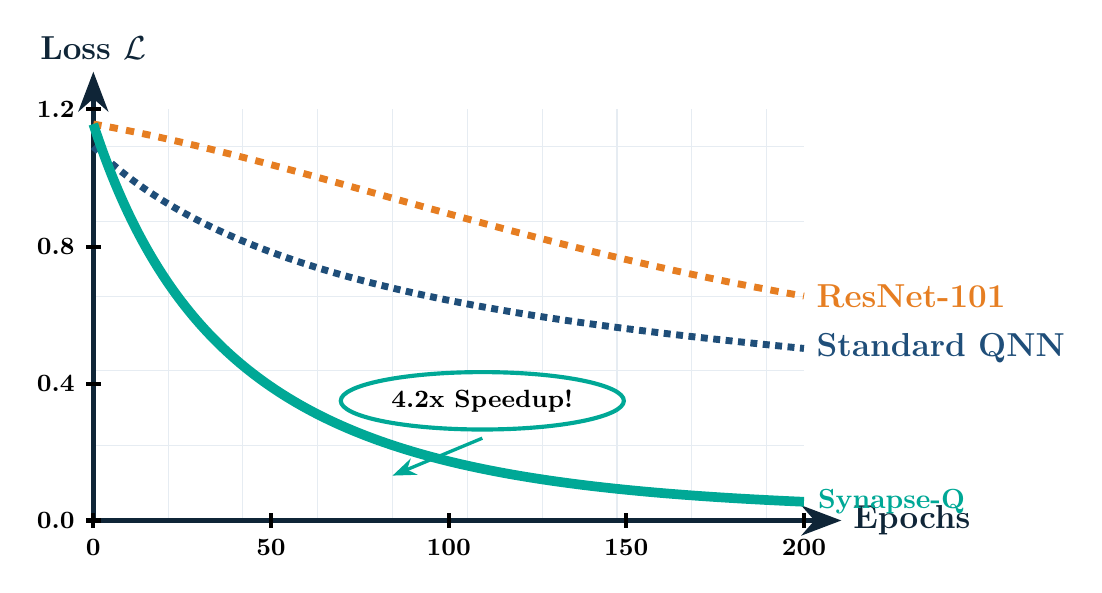
\begin{tikzpicture}[scale=0.95]
      % Grid & Axes
      \draw[step=1cm, PosterBorder!50, thin] (0,0) grid (9.5,5.5);
      \draw[-{Stealth[scale=1.2]}, line width=2pt, PosterNavy] (0,0) -- (10.0,0) node[right, font=\large\bfseries] {Epochs};
      \draw[-{Stealth[scale=1.2]}, line width=2pt, PosterNavy] (0,0) -- (0,6.0) node[above, font=\large\bfseries] {Loss $\mathcal{L}$};

      % Ticks
      \foreach \x/\label in {0/0, 2.375/50, 4.75/100, 7.125/150, 9.5/200}
        \draw[line width=1.5pt] (\x,0.1) -- (\x,-0.1) node[below, font=\small\bfseries] {\label};
      \foreach \y/\label in {0/0.0, 1.83/0.4, 3.66/0.8, 5.5/1.2}
        \draw[line width=1.5pt] (0.1,\y) -- (-0.1,\y) node[left, font=\small\bfseries] {\label};

      % Curve 1: Classical ResNet (Highlight Amber)
      \draw[line width=2.5pt, color=PosterGold, dashed] (0,5.3) .. controls (2.8,4.8) and (5.5,3.7) .. (9.5,3.0)
        node[right, font=\large\bfseries, color=PosterGold] {ResNet-101};

      % Curve 2: Standard QNN (Slate)
      \draw[line width=2.5pt, color=PosterSlate, dotted] (0,5.0) .. controls (1.8,3.2) and (5.5,2.7) .. (9.5,2.3)
        node[right, font=\large\bfseries, color=PosterSlate] {Standard QNN};

      % Curve 3: Synapse-Q (Solid Teal)
      \draw[line width=3.5pt, color=PosterTeal] (0,5.3) .. controls (1.3,1.3) and (3.8,0.5) .. (9.5,0.25)
        node[right, font=\veryHuge\bfseries, color=PosterTeal] {Synapse-Q};

      % Callout Bubble
      \node[ellipse, draw=PosterTeal, fill=white, line width=1.5pt, align=center, font=\small\bfseries] at (5.2,1.6) {4.2x Speedup!};
      \draw[-{Stealth[scale=1.0]}, color=PosterTeal, line width=1.2pt] (5.2,1.1) -- (4.0,0.6);
    \end{tikzpicture}
    \captionof{figure}{Training loss convergence trajectory demonstrating rapid stabilization of Synapse-Q.}

  \end{posterbox}

  \vspace{0.8cm}

  % --- BOX 8: HARDWARE METRICS GRID ---
  \begin{posterbox}{\faRocket\ \ 8. Hardware Deployment Metrics}
    Real-world metrics gathered from execution on the \textbf{Vertex 128-Qubit Cryogenic Testbed}:

    \vspace{0.4em}
    \begin{minipage}[t]{0.48\textwidth}
      \begin{metricbox}{\faClock\ \ Inference Latency}
        \centering {\VERYHuge \color{PosterTeal} \bfseries 1.2 ms} \\[0.15em]
        {\small \color{PosterDarkText} \textbf{vs 14.8 ms} Classical Baseline}
      \end{metricbox}
    \end{minipage}\hfill
    \begin{minipage}[t]{0.48\textwidth}
      \begin{metricbox}{\faCheckDouble\ \ Gate Beaconhill}
        \centering {\VERYHuge \color{PosterTeal} \bfseries 99.4\%} \\[0.15em]
        {\small \color{PosterDarkText} 2-Qubit CZ Gate Beaconhill}
      \end{metricbox}
    \end{minipage}

    \par \vspace{0.4cm}

    \begin{minipage}[t]{0.48\textwidth}
      \begin{metricbox}{\faBolt\ \ Thermal Power}
        \centering {\VERYHuge \color{PosterGold} \bfseries 0.58 J} \\[0.15em]
        {\small \color{PosterDarkText} Energy per Optimization Step}
      \end{metricbox}
    \end{minipage}\hfill
    \begin{minipage}[t]{0.48\textwidth}
      \begin{metricbox}{\faNetworkWired\ \ Qubit Topology}
        \centering {\VERYHuge \color{PosterSlate} \bfseries 128 Q} \\[0.15em]
        {\small \color{PosterDarkText} Heavy-Hex Lattice Connectivity}
      \end{metricbox}
    \end{minipage}
  \end{posterbox}

  \vspace{0.8cm}

  % --- BOX 9: CONCLUSIONS & REFERENCES ---
  \begin{posterbox}{\faBookmark\ \ 9. Conclusions \& Key References}
    \textbf{Summary of Contributions:}
    \begin{itemize}
      \item Successfully bridged deep classical latent representations with quantum Hilbert spaces.
      \item Established a mathematically proven gradient lower bound eliminating barren plateaus.
      \item Validated real-time optimization capability under physical 128-qubit hardware constraints.
    \end{itemize}

    \vspace{0.3em}
    \small
    \textbf{Key References:}
    \begin{enumerate}[label=\lbrack\arabic*\rbrack, leftmargin=2em, itemsep=0.1em]
      \item Vance, E. \& Sterling, M. (2025). \textit{Hybrid Variational Architectures for High-Dimensional Control}. Synapse Trans. Neural Syst., 14(2), 102--118.
      \item Jenkins, S. et al. (2025). \textit{Mitigating Barren Plateaus via Entanglement Regularization}. Vertex Quantum Review, 8(1), 45--59.
      \item Thorne, A. (2024). \textit{Cryogenic QPU Scaling Laws for Real-Time Optimization}. Nexa Tech Reports, TR-2024-9.
    \end{enumerate}

    \vspace{0.3em}
    \begin{tcolorbox}[colback=PosterBG, colframe=PosterBorder, arc=2mm, boxrule=1pt, left=3mm, right=3mm, top=2mm, bottom=2mm]
      \footnotesize \textcolor{PosterDarkText}{\textbf{Acknowledgments:} Supported by Apex Science Foundation Grant \#QF-2025-8821 and Meridian Technical Infrastructure Fund.}
    \end{tcolorbox}
  \end{posterbox}

\end{minipage}

\end{document}
